%================================================
% PACKAGES AND THEMES
%================================================
\documentclass[t,aspectratio=169,xcolor=dvipsnames]{beamer}

\usetheme{SimplePlusAIC}

\usepackage{graphicx}
\usepackage{booktabs}
\usepackage{svg}
\usepackage{tcolorbox}
\usepackage{tikz}
\usepackage{makecell}

\newcommand*{\defeq}{\stackrel{\text{def}}{=}}
\usepackage{setspace}
\usepackage[T1]{fontenc}
\usepackage{helvet}
\usepackage{textgreek}
\usepackage{amsmath}
\usepackage{bm}
\usepackage{ragged2e}
\usepackage{xfrac}
\usepackage[loose]{units}
\usepackage{braket}
\usepackage{physics}
\usepackage{gensymb}
\usepackage{verbatim}
\usepackage{fancyvrb}

\usepackage[svgnames,table]{xcolor}
\arrayrulecolor{black}
\setlength{\arrayrulewidth}{0.20mm}
\renewcommand{\arraystretch}{1.35}

\newcommand{\tem}[1]{\textbf{\textcolor{red}{#1}}}

%================================================
% TITLE PAGE
%================================================
\title[Workshop Sesi 1]{Pemrosesan Bahasa Alami}
\subtitle{PyCaret AutoML for NLP}
\author[SD25-32202]{Martin Manullang}
\institute[ITERA]{Institut Teknologi Sumatera \\ mctm.web.id}
\titlegraphic{\vspace{-0.5cm}
\includegraphics[width=2.5cm]{logos/pycaret.png}}
\date{\textcolor{nyublue}{2026}}

%================================================
% AT BEGIN SECTION - SECTION SEPARATOR
%================================================
\AtBeginSection[]{
  \begin{frame}[plain,c]
    \begin{center}
      \begin{tcolorbox}[
        colback=nyublue!10!white, 
        colframe=nyublue, 
        boxrule=1.5mm, 
        arc=3mm, 
        halign=center,
        valign=center,
        height=0.45\textheight,
        width=0.85\textwidth
      ]
        \Huge\textbf{\textcolor{nyublue}{\insertsectionhead}}
      \end{tcolorbox}
    \end{center}
  \end{frame}
}

%================================================
% BEGIN DOCUMENT
%================================================
\begin{document}

\begin{frame}
    \titlepage
\end{frame}

\begin{frame}
    \frametitle{OUTLINE}
    \framesubtitle{Peta materi pertemuan ini}
    \small
    \begin{spacing}{1.15}
        \tableofcontents
    \end{spacing}
\end{frame}

\begin{frame}
    \frametitle{Capaian Pembelajaran}
    \framesubtitle{Tujuan setelah pertemuan selesai}
    \small
    \begin{enumerate}
        \item Memahami konsep dasar \textit{pipeline} NLP pada Machine Learning tradisional.
        \item Mampu melakukan tahapan ekstraksi fitur dari teks (\textit{TF-IDF} / \textit{Bag of Words}).
        \item Memahami penerapan AutoML menggunakan \texttt{pycaret} untuk teks.
        \item Mampu mengevaluasi model \textit{traditional ML} pada kasus klasifikasi teks.
    \end{enumerate}
    \begin{exampleblock}{Fokus Kelas Ini}
        Kita akan berfokus pada pendekatan \textit{hands-on} dan logika arsitektur modular, \tem{menghindari boilerplate code} yang berlebihan.
    \end{exampleblock}
\end{frame}

\begin{frame}
    \frametitle{Disclaimer}
    \begin{alertblock}{Peringatan Konten SARA \& Eksplisit}
        Studi kasus pada pembelajaran kali ini menggunakan data obrolan interaksi nyata pengguna gim daring (\textit{online game}).
        Oleh karena itu, Dataset yang digunakan mungkin akan memuat kata-kata \textbf{SARA, slang, kata-kata rasis}, dan bahasa yang \textbf{tidak pantas}.
        \vspace{0.2cm}
        
        Materi ini murni digunakan untuk tujuan edukasi dan penelitian pemrosesan bahasa alami.
    \end{alertblock}
\end{frame}

\section{Stack Teknologi \& Arsitektur}

\begin{frame}
    \frametitle{Stack Teknologi}
    \framesubtitle{Library yang akan digunakan}
    \small
    Pendekatan: \textbf{Traditional Machine Learning via AutoML}
    \vspace{0.3cm}
    \begin{itemize}
        \item \textbf{\texttt{pycaret}}: Untuk \textit{training}, komparasi, dan evaluasi model secara instan.
        \item \textbf{\texttt{pandas}}: Untuk manipulasi dan eksplorasi data.
        \item \textbf{\texttt{re} / \texttt{nltk} / \texttt{Sastrawi}}: Untuk \textit{custom text preprocessing} khusus bahasa Indonesia.
    \end{itemize}
\end{frame}

\begin{frame}
    \frametitle{Arsitektur Kode Berbasis Modul}
    \framesubtitle{Pemisahan Core Logic dan Viewer}
    \small
    Kita \textbf{tidak akan} menumpuk eksekusi kode di dalam satu Jupyter Notebook.
    \begin{columns}[T]
        \column{0.48\textwidth}
        \begin{block}{File \texttt{.py} (Core Logic)}
            Seluruh logika ekstraksi, inisialisasi \texttt{pycaret}, komparasi, dan ekspor model.
            \begin{itemize}
                \item \texttt{config.py}
                \item \texttt{preprocess.py}
                \item \texttt{train.py}
            \end{itemize}
        \end{block}

        \column{0.48\textwidth}
        \begin{alertblock}{File \texttt{.ipynb} (Runner \& Viewer)}
            Hanya difungsikan sebagai \textit{runner} presentasi. Memanggil modul \texttt{.py} dalam satu baris, dan menampilkan tabel atau plot grafik hasil.
        \end{alertblock}
    \end{columns}
\end{frame}

\section{Pengenalan PyCaret}

\begin{frame}
    \frametitle{1. Apa itu PyCaret?}
    \small
    \textbf{PyCaret} adalah \textit{framework open-source} berbasis Python dengan konsep \textit{low-code} untuk memfasilitasi \textit{Automated Machine Learning} (AutoML).
    \vspace{0.2cm}
    \begin{itemize}
        \item \textbf{Pengembang Utama}: Diciptakan dan dipelihara oleh \textbf{Moez Ali} sejak tahun 2019.
        \item \textbf{Tujuan Pokok}: Mengotomatiskan eksperimen \textit{machine learning end-to-end}. Mulai dari preparasi data otomatis, \textit{training}, komparasi, \textit{hyperparameter tuning}, analisis \textit{metrics}, hingga ekspor / \textit{deployment}.
    \end{itemize}
    \vspace{0.3cm}
    \begin{center}
        
\includegraphics[width=3cm]{logos/pycaret.png}
    \end{center}
\end{frame}

\begin{frame}
    \frametitle{2. Mengapa PyCaret Sangat Membantu?}
    \small
    \begin{itemize}
        \item \textbf{Low-Code Efficiency}: Secara drastis dapat menggantikan ratusan hingga ribuan baris kode \textit{boilerplate} hanya dengan hitungan 1 atau 2 baris \textit{syntax}.
        \item \textbf{Produktivitas Eksperimen}: Eksperimen puluhan model komparasi algoritma kompleks dari beragam basis librari (\texttt{sklearn}, \texttt{xgboost}, \texttt{catboost}) bisa berjalan instan.
        \item \textbf{Dinding Keamanan Standar}: Praktik pipelining bawaannya mampu mencegah bahaya laten ML sepert \textit{data leakage} dan anomali konversi selama rotasi \textit{K-Fold Cross-Validation}.
        \item \textbf{Berorientasi Solusi (\textit{Beginner Friendly})}: Pengguna /  \textit{Data Scientist} dapat terfokus meneliti kehandalan interpretasi ketimbang pusing mengecor konstruksi algoritma.
    \end{itemize}
\end{frame}

\begin{frame}
    \frametitle{3. Fitur Utama \& Cakupan Algoritma}
    \small
    \textbf{Sistem Fundamental Eksperimen PyCaret}:
    \begin{enumerate}
        \item \texttt{setup()}: Katalisator awal lingkungan. Mentransformasi seluruh vektorisasi teks menjadi data pelatihan siap pakai.
        \item \texttt{compare\_models()}: Arena adu jotos akurasi antarmodel.
    \end{enumerate}
    \vspace{0.2cm}
    \textbf{Ruang Lingkup Estimator (Model Algoritma)}:
    \begin{itemize}
        \item PyCaret memborong banyak algoritma tradisional \textit{state-of-the-art} untuk bertarung secara bersamaan, beberapa \textit{heavy-hitters}-nya antara lain: \textbf{\textit{Light Gradient Boosting Machine}} (\texttt{lightgbm}), \textbf{\textit{Random Forest}} (\texttt{rf}), \textbf{\textit{Decision Tree}} (\texttt{dt}), \textbf{\textit{Support Vector Machines}} (\texttt{svm}), \textbf{\textit{K-Nearest Neighbors}} (\texttt{knn}).
    \end{itemize}
\end{frame}

\section{Dataset}

\begin{frame}
    \frametitle{Detail Dataset NLP}
    \framesubtitle{Indonesian Chat Dataset (Roblox \& Minecraft)}
    \small
    \textbf{Sumber}: Kaggle (\textit{Indonesian Chat Dataset})\\
    \textbf{Karakteristik Teks}: Obrolan \textit{gamer} yang \textbf{kotor}. Penuh dengan \textit{leetspeak}, singkatan ekstrem, dan \textit{slang} lokal.
    
    \vspace{0.2cm}
    \textbf{Informasi Dataset}:
    \begin{itemize}
        \item \textbf{Ukuran dataset}: 10.702 baris $\times$ 3 kolom
        \item \textbf{Kolom}: \texttt{['id', 'chat', 'label']}
    \end{itemize}
    
    \vspace{0.2cm}
    \textbf{Tugas: Multiclass Classification (Distribusi Label)}
    \begin{itemize}
        \item \texttt{violence} \hspace{0.4cm}: 2.983 (27.9\%)
        \item \texttt{neutral} \hspace{0.55cm}: 2.729 (25.5\%)
        \item \texttt{racist} \hspace{0.75cm}: 2.506 (23.4\%)
        \item \texttt{harassment} \hspace{0.1cm}: 2.484 (23.2\%)
        \item \textbf{TOTAL} \hspace{0.75cm}: \textbf{10.702 baris}
    \end{itemize}
\end{frame}

\begin{frame}
    \frametitle{Contoh Data}
    \small
    Berikut adalah cuplikan data teratas:
    \vspace{0.2cm}
    \begin{table}[]
        \resizebox{\textwidth}{!}{
        \begin{tabular}{@{}c p{12cm} l@{}}
        \toprule
        \textbf{id} & \textbf{chat} & \textbf{label} \\ \midrule
        0 & main mu kek tai cok & violence \\
        1 & user telat ngasih tau elu edan sarap gue bergaul elu & violence \\
        2 & kadang berfikir percaya tuhan jatuh berkalikali kadang tuhan ninggalkan oran... & neutral \\
        3 & user user aku\textbackslash n\textbackslash nku tau matamu sipit diliat & racist \\
        4 & capek deh ketemu kaum cina kapir gini match & racist \\ \bottomrule
        \end{tabular}
        }
    \end{table}
\end{frame}

\section{Teori Preprocessing Teks}

\begin{frame}
    \frametitle{1. Apa itu Text Preprocessing?}
    \framesubtitle{Mengapa teks harus dibersihkan?}
    \small
    \textbf{Text Preprocessing} adalah tahapan krusial dalam NLP untuk mengubah teks mentah menjadi format yang dapat dipahami oleh model \textit{Machine Learning}.
    
    \vspace{0.3cm}
    \textbf{Alasan Utama}:
    \begin{itemize}
        \item Teks dari internet (terutama \textit{chat}) penuh dengan "noise".
        \item Komputer tidak memahami teks alfabetikal, melainkan \textbf{angka}.
        \item Teks yang bersih akan \textbf{mengurangi dimensi fitur} (jumlah kata unik) secara sangat drastis dan \textbf{meningkatkan akurasi} model.
        \item Prinsip \textit{"Garbage In, Garbage Out"} - Sebaik apapun algoritma komparasi, jika kualitas teks buruk maka hasil prediksi gagal.
    \end{itemize}
\end{frame}

\begin{frame}
    \frametitle{2. Tahapan Klasik Preprocessing Teks}
    \small
    Secara teori, alur pembersihan teks tradisional seringkali melewati 6 langkah berikut secara berurutan:
    \vspace{0.3cm}
    \begin{enumerate}
        \item \textbf{Text Cleaning} (Pembersihan Teks Dasar)
        \item \textbf{Normalization / Slang Words Handling} (Normalisasi)
        \item \textbf{Tokenization} (Tokenisasi)
        \item \textbf{Stopword Removal} (Penyaringan Stopword)
        \item \textbf{Stemming / Lemmatization} (Pencarian Kata Dasar)
        \item \textbf{Text Representation / Vectorization} (Vektorisasi TF-IDF)
    \end{enumerate}
\end{frame}

\begin{frame}
    \frametitle{3. Text Cleaning (Pembersihan Awal)}
    \framesubtitle{Lowercasing \& Punctuation Removal}
    \small
    \textbf{Lowercasing}
    \begin{itemize}
        \item Mengubah semua huruf menjadi huruf kecil.
        \item Menyeragamkan kosakata: "Toxic", "TOXIC", dan "toxic" akan digabungkan menjadi satu identitas variabel kata.
        \item \textit{Contoh}: "DASAR NOOB!" $\rightarrow$ "dasar noob!"
    \end{itemize}
    
    \vspace{0.3cm}
    \textbf{Punctuation \& Special Character Removal}
    \begin{itemize}
        \item Menghapus tanda baca (!, ?, ., ,) dan karakter emoji / simbol ASCII.
        \item Karakter non-alfabet terkadang jarang memiliki makna prediktif kuat pada ML Tradisional (\textit{Term Frequency}).
        \item \textit{Contoh}: "halo!!! apa kabar??" $\rightarrow$ "halo apa kabar"
    \end{itemize}
\end{frame}

\begin{frame}
    \frametitle{4. Text Cleaning (Lanjutan)}
    \framesubtitle{Menangani URL, Mention, dan Hashtag}
    \small
    Data media sosial/gim sering memuat elemen teknis sistem yang tidak memiliki makna leksikal \textit{human-language}:
    \vspace{0.2cm}
    \begin{itemize}
        \item \textbf{Menghapus URL/Link}: Tautan situs seperti \texttt{http://...} atau \texttt{www.} dihapus karena merupakan \textit{noise} mutlak.
        \item \textbf{Menghapus Mention}: Kata yang diawali \texttt{@}. Biasanya dinormalisasi menjadi token netral \textbf{[USER]}. \textit{Di dataset kita, hal ini sudah disensor menjadi kata "user"}.
        \item \textbf{Menangani Hashtag}: Tanda \texttt{\#} dihapus namun teksnya dipertahankan, karena misal kata \texttt{\#boikot} bermakna penting dalam teks opini.
    \end{itemize}
\end{frame}

\begin{frame}
    \frametitle{5. Normalization \& Slang Handling}
    \framesubtitle{Tantangan Teks Gamer \& Media Sosial}
    \small
    Data chat tidak menggunakan bahasa baku. Tahap ini sangat krusial:
    \vspace{0.2cm}
    \begin{itemize}
        \item \textbf{Leetspeak Transformation}: Memetakan kata beralfanumerik ke abjad absolut.
        \begin{itemize}
            \item \textit{Contoh}: "m4k4n" $\rightarrow$ "makan", "b99" $\rightarrow$ "bangg"
        \end{itemize}
        \item \textbf{Repeated Characters Removal}: Memotong karakter yang memanjang tidak wajar (\textit{elongated words}).
        \begin{itemize}
            \item \textit{Contoh}: "noooobbbb bangggeetttt" $\rightarrow$ "noob banget"
        \end{itemize}
        \item \textbf{Slang Dictionary Mapping}: Kamus pemetaan manual (\textit{alay map}) untuk memperbaiki ejaan.
        \begin{itemize}
            \item \textit{Contoh}: "yg", "sgt", "kuy" $\rightarrow$ "yang", "sangat", "ayo"
        \end{itemize}
    \end{itemize}
\end{frame}

\begin{frame}
    \frametitle{6. Tokenization}
    \framesubtitle{Pemecahan Teks Menjadi Unit Kecil}
    \small
    \textbf{Tokenization} adalah proses memecah kalimat utuh menjadi unit-unit individu teks yang lebih diskrit yang disebut dengan \textit{token} (kata).
    
    \vspace{0.2cm}
    \begin{exampleblock}{Contoh Tokenisasi Kata (Word Tokenization)}
        Kalimat: "Bocah ini sangat toxic sekali" \\
        $\rightarrow$ \texttt{["bocah", "ini", "sangat", "toxic", "sekali"]}
    \end{exampleblock}
    
    \vspace{0.2cm}
    Fungsi dari tahap ini adalah agar model (seperti Scikit-Learn atau PyCaret nantinya) dapat menghitung statistik frekuensi tiap kata satu per satu pada tahap representasi vektor.
\end{frame}

\begin{frame}
    \frametitle{7. Stopword Removal}
    \framesubtitle{Menyaring Kata Kebisingan Ekstrim}
    \small
    \textbf{Stopwords} adalah kata-kata sambung atau umum yang frekuensi kemunculannya ekstrim, \textbf{namun} secara semantik tidak membedakan polaritas kelas pada kalimat.
    
    \vspace{0.2cm}
    \begin{itemize}
        \item \textbf{Contoh (Indonesia)}: "yang", "dan", "di", "ke", "dari", "ini", "itu".
        \item Menghapus stopwords akan memangkas dimensi memori pelatihan algoritma secara dramatis tanpa mengorbankan konteks klasifikasi.
    \end{itemize}
    
    \vspace{0.2cm}
    \begin{alertblock}{Contoh Filtering Stopword}
        \textbf{Awal}: \texttt{["saya", "ingin", "makan", "di", "restoran", "itu"]} \\
        \textbf{Akhir}: \texttt{["makan", "restoran"]}
    \end{alertblock}
\end{frame}

\begin{frame}
    \frametitle{8. Stemming vs Lemmatization}
    \framesubtitle{Dua Pendekatan Mengurai Imbuhan}
    \small
    Tujuannya yaitu memadatkan atau menyatukan variasi dan variabilitas imbuhan menjadi 1 representasi kata dasar.
    \vspace{0.2cm}
    \begin{columns}[T]
        \column{0.48\textwidth}
        \textbf{Stemming}
        \begin{itemize}
            \item Memotong otomatis awalan/akhiran menggunakan \textit{heuristic rules} (kasar).
            \item Sangat ringkas, cepat, namun hasil katanya bisa tidak memiliki arti.
            \item \textit{memperbaiki} $\rightarrow$ \textit{baik}
        \end{itemize}
        
        \column{0.48\textwidth}
        \textbf{Lemmatization}
        \begin{itemize}
            \item Resolusi leksikal analisis kamus dan morfologi kata asal (lemma).
            \item Sangat komputasional / lambat, ekstensif gramatikal, tapi \textit{100\% valid}.
            \item \textit{better} $\rightarrow$ \textit{good}
        \end{itemize}
    \end{columns}
\end{frame}

\begin{frame}
    \frametitle{9. Dilema Stemming Bahasa Indonesia}
    \framesubtitle{Mekanik \textit{Library} Sastrawi}
    \small
    Bahasa Indonesia memiliki morfologi rumit. \textit{Lemmatization} sangat berat diterapkan karena minimnya ketersediaan NLP teroptimasi.
    \vspace{0.2cm}
    \begin{itemize}
        \item Peneliti Python lokal menggunakan \textit{library} \textbf{Sastrawi} / \textbf{PySastrawi} untuk urusan \textbf{Stemming} Indonesia.
        \item Implementasinya mengacu pada turunan algoritma \textit{Nazief \& Adriani}.
        \item \textbf{Permasalahannya} pada kasus dataset gamer / chat \textit{slang}: Stemmer formal gagal melakukan stemming pada kalimat yang bukan bahasa baku / KBBI. Oleh sebab itu penanganan slang wajib di nomor satu-kan.
    \end{itemize}
\end{frame}

\begin{frame}
    \frametitle{10. Text Feature Representation}
    \framesubtitle{Bag of Words \& TF-IDF}
    \small
    Seketika preprocessing selesai, hasil akhir corpus masuk ke babak matematis mengubah tokenisasi vektor huruf $\rightarrow$ menjadi angka riil desimal.
    \vspace{0.2cm}
    \begin{itemize}
        \item \textbf{Bag of Words (BoW)}: Mendata total statistik frekuensi setiap kosakata dokumen. \textit{Term yang paling sering tampil memegang kendali terbanyak, mengabaikan konteks di kalimat lain.}
        \item \textbf{TF-IDF} (\textit{Term Frequency - Inverse Document Frequency}): 
        Algoritma standar industri untuk menskor (rating) pada kata.
        \begin{itemize}
            \item Misal, kosakata obrolan X sering muncul kuat di baris "toxic", \textbf{TAPI JARANG} diutarakan pemain di baris netral, nilai kata itu \textbf{dikali berlipat ganda karena ia merupakan kata unik per kelas.}
        \end{itemize}
    \end{itemize}
\end{frame}

\section{Alur Pipeline}

\begin{frame}
    \frametitle{Tahapan Pipeline (1-2)}
    \framesubtitle{Dari Pembersihan ke Setup}
    \small
    \begin{enumerate}
        \item \textbf{Custom Text Cleaning}
        \begin{itemize}
            \item Teks \textit{gamer} butuh pembersihan khusus.
            \item Menangani \textit{leetspeak} angka dan \textit{slang} agar kata-kata tidak terbuang atau kehilangan maknanya.
        \end{itemize}
        \vspace{0.2cm}
        \item \textbf{AutoML Setup}
        \begin{itemize}
            \item Menggunakan \texttt{pycaret.classification.setup}.
            \item Konfigurasi setup untuk melakukan transformasi \textit{TF-IDF} (\textit{Term Frequency - Inverse Document Frequency}) secara otomatis.
        \end{itemize}
    \end{enumerate}
\end{frame}

\begin{frame}
    \frametitle{1. Bedah Fungsi \texttt{setup()}}
    \framesubtitle{Gerbang Utama Eksperimen}
    \small
    Fungsi \texttt{setup()} adalah langkah terpenting dalam PyCaret yang wajib diinisialisasi pertama kali.
    \vspace{0.3cm}
    \begin{itemize}
        \item \textbf{Fungsi Pokok}: Mengambil variabel dataframe \textit{pandas} dan merekayasa skema lingkungan ML secara absolut.
        \item Mengelola strategi \textit{train-test split} secara adil dengan menyamakan rasio distribusi kelas minoritas dan mayoritas (\textit{Stratified K-Fold}).
        \item Mentransformasi fitur teks menjadi numerik berdimensi tinggi sebelum dikonsumsi oleh algoritma menggunakan \textit{TF-IDF text embedding}.
    \end{itemize}
\end{frame}

\begin{frame}
    \frametitle{2. Hyperparameter pada \texttt{setup()} (1/2)}
    \framesubtitle{Konfigurasi Inti \& Teks}
    \scriptsize
    Dalam PyCaret, fungsi \texttt{setup()} memiliki belasan argumen. Berikut beberapa konfigurasi penting:
    \vspace{0.2cm}
    \begin{columns}[T]
        \column{0.48\textwidth}
        \begin{block}{Parameter Wajib}
            \begin{itemize}
                \item \texttt{data=df\_chat} $\rightarrow$ Mendeklarasikan sumber *dataset* dari objek \textit{pandas} di memori.
                \item \texttt{target='label'} $\rightarrow$ Menentukan nama spesifik kolom yang ingin diprediksi klasifikasinya.
            \end{itemize}
        \end{block}
        \begin{block}{Parameter Reproducibility}
            \begin{itemize}
                \item \texttt{session\_id=42} $\rightarrow$ Mengunci \textit{random seed state} agar pembagian acak konsisten (\textit{reproducible}) setiap kali *code* dijalankan di mesin siapapun.
            \end{itemize}
        \end{block}

        \column{0.48\textwidth}
        \begin{block}{Parameter Fitur Teks Khusus NLP}
            \begin{itemize}
                \item \texttt{text\_features=['chat']} $\rightarrow$ Memberitahu mesin tentang eksistensi kolom berisi teks paragraf mentah yang wajib dibedah.
                \item \texttt{text\_features\_embedding\_\\method='tf-idf'} $\rightarrow$ Menugaskan ekstraktor algoritma TF-IDF (*Term Frequency Inverse Document Frequency*) ke kolom teks di atas. (\textit{Bisa diubah ke 'bow' untuk sekadar hitung frekuensi kemunculan}).
            \end{itemize}
        \end{block}
    \end{columns}
\end{frame}

\begin{frame}
    \frametitle{3. Hyperparameter Lanjutan \texttt{setup()} (2/2)}
    \framesubtitle{Strategi Validasi, Hardware, \& Preprocessing Ekstra}
    \scriptsize
    \begin{columns}[T]
        \column{0.48\textwidth}
        \begin{block}{Strategi Training \& Hardware}
            \begin{itemize}
                \item \texttt{train\_size=0.8} $\rightarrow$ Porsi pemisahan data latih (80\%) vs data uji rahasia (20\%).
                \item \texttt{fold=5} \& \texttt{fold\_strategy='stratified'} $\rightarrow$ Memecah validasi silang (CV) rata pada semua lipatan kelas.
                \item \texttt{use\_gpu=True} $\rightarrow$ Mengalihkan \textit{workload} matematika tensor ekstrim ke RAM Kartu Grafis (NVIDIA/CUDA).
                \item \texttt{n\_jobs=-1} $\rightarrow$ Mengerahkan paksa efisiensi 100\% utilitas \textit{core thread} CPU spesifikasi server.
            \end{itemize}
        \end{block}

        \column{0.48\textwidth}
        \begin{alertblock}{Parameter \textit{Secret Weapon} Lainnya}
            PyCaret sanggup menyulap manipulasi data tingkat dewa hanya dengan mengatur bendera (\textit{flags}):
            \begin{itemize}
                \item \texttt{normalize=True} $\rightarrow$ Meratakan rasio skala simpangan baku fitur numerik ekstrem \textit{(Z-Score / MinMax)}.
                \item \texttt{pca=True} $\rightarrow$ Mengompresi dimensi kolom ribuan teks (TF-IDF) jadi puluhan vektor utama (\textit{Dimensionality Reduction}).
                \item \texttt{fix\_imbalance=True} $\rightarrow$ Otomatis menduplikasi (\textit{Oversampling} SMOTE) target kelas dataset yang jumlah minoritasnya menyedihkan!
                \item \texttt{ignore\_features=['id']} $\rightarrow$ Membutakan model dari kolom irrelevan agar tidak ikut difiturisasi.
            \end{itemize}
        \end{alertblock}
    \end{columns}
\end{frame}

\begin{frame}
    \frametitle{3. Membaca Output Tabel \texttt{setup()} (Bagian 1)}
    \small
    Saat \texttt{setup()} dieksekusi, panel *dashboard* teratas akan memberi laporan parameter komputasi. Parameter terpenting antara lain:
    \vspace{0.2cm}
    \begin{itemize}
        \item \textbf{Target type} (Multiclass): Sistem otomatis mendeteksi total kategori label target melebihi dari 2 variasi kelas (\textit{binary}).
        \item \textbf{Target mapping}: \texttt{\{harassment: 0, neutral: 1, racist: 2, violence: 3\}}. Otomatis (*One-Hot Encoder*) menyandi label teks menjadi nominal (0-3).
        \item \textbf{Original data shape}: Total ukuran keranjang awal \textbf{(10.702 baris, 2 kolom)}.
        \item \textbf{Transformed data shape}: Menjadi \textbf{(10.702 baris, 18.117 kolom fitur)}! Ukuran ruang ini meledak murni dari *vocabulary token* karena pemrosesan TF-IDF kata. Tiap sel menampung frekuensi \textit{rating}!
    \end{itemize}
\end{frame}

\begin{frame}
    \frametitle{4. Membaca Output Tabel \texttt{setup()} (Bagian 2)}
    \small
    \begin{itemize}
        \item \textbf{Transformed train set shape}: Menyerap \textbf{8.561} obrolan ke ring (80\% data primer \textit{train} untuk menggembleng "kerangka otak" model).
        \item \textbf{Transformed test set shape}: Mengunci rahasia sisa proporsi \textbf{2.141} obrolan (20\% hold-out). Pintu \textit{test set} ini haram hukumnya dilihat algoritma ketika masa *training*, berfungsi vital sebagai soal ujian murni objektif.
        \item \textbf{Fold Generator} (StratifiedKFold): Memastikan lipatan per kelas imbang.
        \item \textbf{Use GPU} (True): Mengalirkan iterasi pembagian tensor NLP dan algoritma tangguh lewat unit prosesor sentral grafis VRAM (misal CUDA) yang jauh melampaui paralelisasi CPU biasa.
    \end{itemize}
\end{frame}

\begin{frame}
    \frametitle{5. Konsep 5-Fold Cross Validation}
    \framesubtitle{Mengapa tidak cukup 1 kali training?}
    \small
    Dalam parameter awal, kita mengatur sistem siklus ditiup menjadi 5 balikan rotasi (\texttt{Fold=5}).
    \vspace{0.2cm}
    \begin{itemize}
        \item \textbf{Prinsip}: Data primer *train set*\textbf{ dibagi / di-iris adil jadi 5 patahan}. 
        \item Model melatih pengetahuannya pada \textbf{4 patahan awal}, lalu dihantam \textit{ujian rahasia} mendadak di \textbf{1 patahan sisa} ujung. 
        \item \textbf{Proses ini digulirkan \& diulang} dengan pergantian posisi peta \textit{training} yang terus bergeser.
        \item \textbf{Tujuan Pokok}: *Machine Learning* tidak boleh hafal lokasi data pola semu. Kemampuannya harus tervalidasi jendral ke dimensi apa pun dalam distribusinya (membuang \textit{over-lucky metric} atau bias kebetulan tinggi).
    \end{itemize}
\end{frame}

\begin{frame}
    \frametitle{6. Diagram Visual K-Fold Cross Validation}
    \begin{center}
        \resizebox{0.80\textwidth}{!}{
        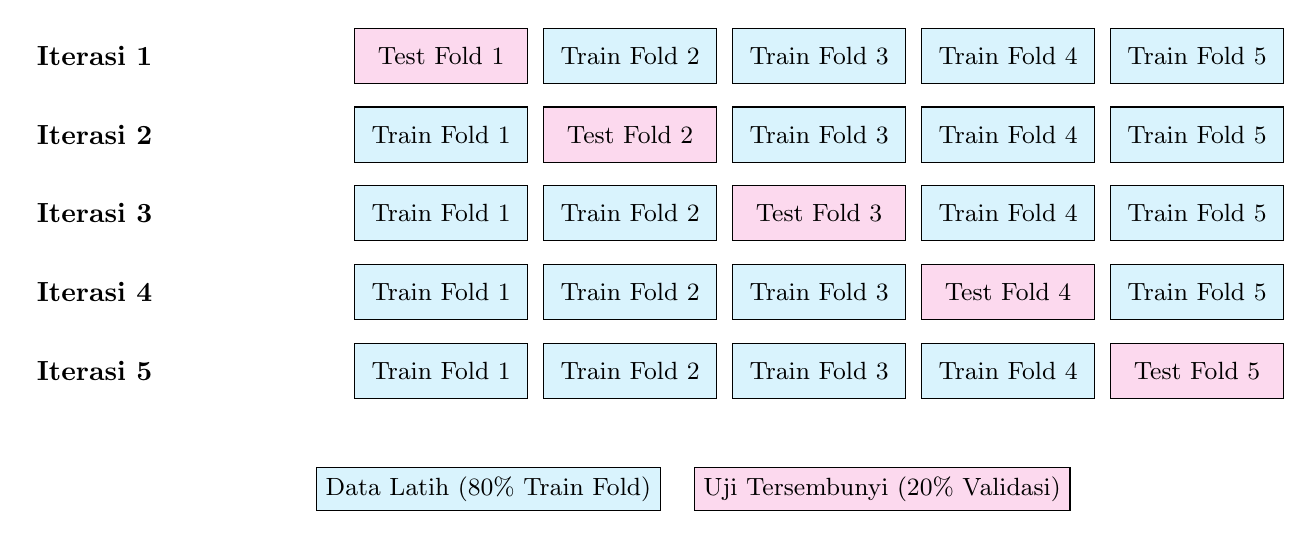
\begin{tikzpicture}[
            fold/.style={rectangle, draw, minimum width=2.2cm, minimum height=0.7cm, align=center},
            train/.style={fold, fill=cyan!15},
            val/.style={fold, fill=magenta!15}
        ]
            % Titles
            \node at (-2, 0) {\textbf{Iterasi 1}};
            \node at (-2, -1) {\textbf{Iterasi 2}};
            \node at (-2, -2) {\textbf{Iterasi 3}};
            \node at (-2, -3) {\textbf{Iterasi 4}};
            \node at (-2, -4) {\textbf{Iterasi 5}};
            
            % Folds
            \foreach \y/\v in {0/1, -1/2, -2/3, -3/4, -4/5} {
                \foreach \x in {1,2,3,4,5} {
                    \ifnum\x=\v
                        \node[val] at (\x*2.4, \y) {\small Test Fold \x};
                    \else
                        \node[train] at (\x*2.4, \y) {\small Train Fold \x};
                    \fi
                }
            }
            
            % Legend
            \node[train, minimum width=1.5cm, minimum height=0.4cm] at (3, -5.5) {\small Data Latih ($80\%$ Train Fold)};
            \node[val, minimum width=1.5cm, minimum height=0.4cm] at (8, -5.5) {\small Uji Tersembunyi ($20\%$ Validasi)};
        \end{tikzpicture}
        }
    \end{center}
    \vspace{0.2cm}
    \footnotesize Skor final parameter (*Akurasi, F1*, dll.) keluar sebagai nilai rata-rata (*Mean Out-Of-Fold*) mutlak, dan \textbf{bukan dari iterasi tebakan "terhoki"/terbaiknya}!
\end{frame}

\begin{frame}
    \frametitle{Tahapan Pipeline (3-5)}
    \framesubtitle{Komparasi Model hingga Deployment}
    \small
    \begin{enumerate}
        \setcounter{enumi}{2}
        \item \textbf{Model Arena}
        \begin{itemize}
            \item Membandingkan (\textit{compare}) algoritma tradisional (misal: SVM, CatBoost, LightGBM).
            \item Mencari algoritma dengan Akurasi dan F1-Score teringgi.
        \end{itemize}
        \vspace{0.1cm}
        \item \textbf{Evaluation}
        \begin{itemize}
            \item Menganalisis hasil dari model terbaik.
            \item Melihat pola dari \textit{Confusion Matrix} dan \textit{Feature Importance} (kata apa yang paling memicu suatu label, misal kata untuk \textit{toxic}).
        \end{itemize}
        \vspace{0.1cm}
        \item \textbf{Finalize}
        \begin{itemize}
            \item Membungkus seluruh \textit{pipeline} utuh (preprocessing, vektorisasi TF-IDF, model) menjadi file statis (\texttt{.pkl}).
        \end{itemize}
    \end{enumerate}
\end{frame}

\section{Komparasi Model \& Evaluasi}

\begin{frame}
    \frametitle{1. Tinjauan Algoritma Klasik (DT \& RF)}
    \framesubtitle{Decision Tree \& Random Forest}
    \scriptsize
    Fungsi \texttt{compare\_models()} akan mengadu belasan algoritma. Berikut profil algoritma andalan:
    \vspace{0.2cm}
    \begin{columns}[T]
        \column{0.48\textwidth}
        \begin{block}{\texttt{dt} (Decision Tree)}
            \textbf{Mekanisme}: Membuat aturan \textit{if-then} bercabang seperti algoritma kuesioner \textit{Yes/No} atau Diagram Alir (\textit{Flowchart}).\\
            \vspace{0.2cm}
            \textbf{Kelebihan/Kekuranga}: Pengambilan keputusannya sangat transparan dan \textbf{mudah dimengerti manusia}, namun amat rentan terhadap \textit{overfitting} (terlalu menghafal data letak \textit{training} ketimbang memahami pola asli).\\
            \vspace{0.2cm}
            \colorbox{orange!20}{\textit{Analogi: Seperti bos perfeksionis yang menghafal}}
            \colorbox{orange!20}{\textit{mati prosedur kaku, tapi gagap saat ada kasus baru.}}
        \end{block}

        \column{0.48\textwidth}
        \begin{block}{\texttt{rf} (Random Forest)}
            \textbf{Mekanisme}: Evolusi (*ensemble*) dari DT. Alih-alih 1 pohon rapuh, RF menumbuhkan "hutan" berisi ratusan pohon keputusan berukuran mini secara acak, dan setiap klasifikasi akhir didapat via \textbf{\textit{voting}} (suara terbanyak rata-rata).\\
            \vspace{0.2cm}
            \textbf{Kelebihan}: RF jauh lebih \textbf{stabil dan konsisten}.\\
            \vspace{0.2cm}
            \colorbox{nyublue!20}{\textit{Analogi: Daripada tanya 1 dokter spesialis yang}}
            \colorbox{nyublue!20}{\textit{bisa salah (DT), lebih baik kumpulkan 100 dokter}}
            \colorbox{nyublue!20}{\textit{umum lalu ambil diagnosis suara terbanyak (RF)!}}
        \end{block}
    \end{columns}
\end{frame}

\begin{frame}
    \frametitle{2. Algoritma Jarak \& Pemisah (KNN \& SVM)}
    \scriptsize
    \begin{columns}[T]
        \column{0.48\textwidth}
        \begin{block}{\texttt{knn} (K-Nearest Neighbors)}
            \textbf{Mekanisme}: Menebak sentimen teks baru berdasarkan \textbf{kedekatan jarak grafis} K-jumlah teks "tetangga terdekat"-nya.\\
            \vspace{0.2cm}
            \textbf{Kekurangan Vital}: Pemalas di awal, tapi tersiksa di akhir. Ia \textit{lazy learning} menahan *semua* observasi matematis di memori sehingga performanya \textbf{menurun drastis} dihantam dataset teks lebat.\\
            \vspace{0.2cm}
            \colorbox{orange!20}{\textit{Analogi: Anak gaul yang sifat dan hobinya}}
            \colorbox{orange!20}{\textit{selalu dipengaruhi rata-rata 5 teman tongkrongannya.}}
        \end{block}

        \column{0.48\textwidth}
        \begin{block}{\texttt{svm} (Support Vector Machines)}
            \textbf{Mekanisme}: Menarik garis tembok (\textit{hyperplane}) mutlak sebagai \textbf{jurang pembatas} antar satu label spasial dengan label lainnya secara matematis ekstrim.\\
            \vspace{0.2cm}
            \textbf{Kelebihan Utama}: Sangat \textbf{kokoh, akurat, dan merajai klasifikasi dunia NLP} berskalabilitas tinggi karena tahan banting memproses miliaran dimensi ekstraksi teks TF-IDF.\\
            \vspace{0.2cm}
            \colorbox{nyublue!20}{\textit{Analogi: Membangun rentangan tembok Berlin raksasa}}
            \colorbox{nyublue!20}{\textit{untuk memisahkan kota perusuh vs kota damai.}}
        \end{block}
    \end{columns}
\end{frame}

\begin{frame}
    \frametitle{3. State-of-the-Art: Gradient Boosting}
    \scriptsize
    \begin{columns}[T]
        \column{0.48\textwidth}
        \begin{block}{\texttt{lightgbm} (Light Gradient Boosting Machine)}
            \textbf{Sejarah}: Mahakarya \textit{open-source} inisiatif \textbf{Microsoft} yang sering kali merajai puncak kompetisi AI *Kaggle*. Algoritma level Dewa untuk dataset gajah.\\
            \vspace{0.2cm}
            \textbf{Kehebatan}: Berfokus pada efisiensi optimasi RAM yang sangat pelit (\textit{leaf-wise tree growth}), menjadikannya sangat agresif, brutal, cepat, dengan akurasi terpresisi. Sangat *recommended* untuk AutoML.
        \end{block}

        \column{0.48\textwidth}
        \begin{alertblock}{Rahasia Mekanik (\textit{Boosting})}
            Berbeda dengan \texttt{Random Forest} (RF) yang membina ratusan pohon secara serentak \& independen, metode \textit{Boosting} itu mendidik model secara \textbf{Berantai}.\\
            \vspace{0.2cm}
            Ia membangun 1 pohon awal. Lalu disusul pohon kedua yang secara dramatis dan eksklusif \textbf{hanya difokuskan untuk memperbaiki error kelemahan dari pohon pertama!} Begitu terus menerus.\\
            \vspace{0.2cm}
            \colorbox{yellow!40}{\textit{Analogi: Tim estafet lari di mana pelari kedua}}
            \colorbox{yellow!40}{\textit{mati-matian mengebut guna menutupi}}
            \colorbox{yellow!40}{\textit{keterbelakangan pelari pertama!}}
        \end{alertblock}
    \end{columns}
\end{frame}

\begin{frame}
    \frametitle{4. Membaca Scoring Metrics (Akurasi \& Akal-akalan)}
    \scriptsize
    PyCaret mengurutkan model berdasarkan *Metrics*. Mari kita bedah hati-hati!
    \vspace{0.2cm}
    \begin{columns}[T]
        \column{0.48\textwidth}
        \begin{block}{Accuracy (Akurasi)}
            Mengukur persentase rasio (\%) tebakan model yang benar mutlak.\\
            \vspace{0.2cm}
            \textbf{Awas, Akurasi itu Buta!} Jika data cacat (99\% Netral, 1\% Toxic), model bodoh yang menebak SEMUA teks sebagai Netral akan mendapat akurasi ajaib 99\%, memalsukan kesuksesan evaluasi!
        \end{block}

        \column{0.48\textwidth}
        \begin{block}{AUC (\textit{Area Under the ROC Curve})}
            Menghitung efektivitas model membedakan sebaran dua sisi polaritas kelas agar jangan tumpang tindih.\\
            \vspace{0.2cm}
            \begin{itemize}
                \item Skor \textbf{1.0} $\rightarrow$ Dewa \textit{machine-learning}.
                \item Skor \textbf{0.5} $\rightarrow$ Setara performa melempar koin (kebetulan acak murni).
            \end{itemize}
        \end{block}
    \end{columns}
\end{frame}

\begin{frame}
    \frametitle{5. Precision, Recall, \& F1 Score}
    \framesubtitle{Triumvirate Evaluasi Data Imbalanced}
    \scriptsize
    \begin{columns}[T]
        \column{0.32\textwidth}
        \begin{block}{Precision}
            Dari total yang dituding "Rasis", berapa yang \textbf{benar-benar asli} rasis?\\
            \vspace{0.1cm}
            (Menuntut kehati-hatian sistem menghindari salah tangkap).
        \end{block}

        \column{0.32\textwidth}
        \begin{block}{Recall}
            Dari jangkauan 100 pesan rasis *original*, terjaring \textbf{seberapa luas} oleh model?\\
            \vspace{0.1cm}
            (Menyapu bersih, biarpun *false alarm* ikut diangkut).
        \end{block}
        
        \column{0.34\textwidth}
        \begin{alertblock}{F1 Score}
            Nilai rata-rata penengah (*gold standard*) di antara Recall dan Precision. \textbf{Jadikan skor F1 prioritas utama di kehidupan nyata!}
        \end{alertblock}
    \end{columns}
\end{frame}

\begin{frame}
    \frametitle{6. Contoh Perhitungan: Kasus Kebencian (1/2)}
    \scriptsize
    \textbf{Studi Kasus}: Kita memiliki \textbf{100 chat} ujaran kebencian asli di dalam data rahasia (*Test Set*).
    \begin{columns}[T]
        \column{0.48\textwidth}
        \begin{alertblock}{Skenario A (Super Hati-hati = High Precision)}
            Model A menembak 10 pesan sebagai kebencian.
            \begin{itemize}
                \item Dari 10 tebakan, \textbf{10-nya 100\% BENAR asli}.
                \item \textbf{Precision} = 100\% (Sempurna tidak salah tangkap)
                \item \textbf{Recall} = Namun dari 100 penjahat asli, ia cuma berhasil menjaring 10. (Recall = 10\% - Gagal total melacak sisa 90 penjahat lain!)
            \end{itemize}
        \end{alertblock}

        \column{0.48\textwidth}
        \begin{alertblock}{Skenario B (Super Serok = High Recall)}
            Model B menembak \textbf{200 pesan} sekaligus sebagai kebencian.
            \begin{itemize}
                \item Dari 200 tembakan, ia berhasil mengangkat ke-100 kotoran. \textbf{Recall = 100\%} (Menyapu bersih).
                \item \textbf{Precision} = Total tebak 200, cuma benar 100. (Precision 50\%, artinya setengah warga korbannya ditangkap sembarangan!)
            \end{itemize}
        \end{alertblock}
    \end{columns}
\end{frame}

\begin{frame}
    \frametitle{7. Contoh Perhitungan: Kasus Kebencian (2/2)}
    \scriptsize
    Kita tidak mau model yang kerjanya asal tangkap rakyat (Skenario B), tapi enggan pula mempekerjakan detektif yang gagal melacak sisa pelapor kejahatan (Skenario A). \textbf{Di situlah F1 Score lahir}.
    \vspace{0.2cm}
    \begin{columns}[T]
        \column{0.48\textwidth}
        \begin{block}{Rumus Harfiah F1-Score}
            $F1 = 2 \times \frac{Precision \times Recall}{Precision + Recall}$
        \end{block}
        \textbf{Ilustrasi Hasil Imbang Model C}:
        \begin{itemize}
            \item Model C menebak 110 tebakan kebencian.
            \item Ia berhasil menangkap 90 kotoran murni (Recall \textbf{90\%}).
            \item Dari 110 tembakan, meleset 20 ke orang tak bersalah (Precision: 90 / 110 = \textbf{81.8\%}).
        \end{itemize}

        \column{0.48\textwidth}
        \begin{block}{Putusan PyCaret}
            \textbf{Skor F1} Model C:
            = $2 \times \frac{0.818 \times 0.90}{0.818 + 0.90} \approx \textbf{0.85}$ (atau 85\%)\\
            \vspace{0.2cm}
            \textit{Data Scientist} akan selalu memperebutkan dan memenangkan Model C di turnamen karena performa keseimbangannya yang jauh lebih realistis!
        \end{block}
    \end{columns}
\end{frame}

\begin{frame}
    \frametitle{8. Indikator Tambahan (Kappa, MCC, TT)}
    \scriptsize
    \begin{columns}[T]
        \column{0.48\textwidth}
        \begin{block}{Kappa \& MCC (\textit{Matthews Correlation Coefficient})}
            Variasi *scoring threshold* penyeimbang perhitungan "kebetulan asal tebak dadu", amat kebal rentetan kelas data miring.
            \begin{itemize}
                \item Nilai \textbf{1.0} $\rightarrow$ Sempurna mutlak.
                \item Nilai $\leq$ \textbf{0.0} $\rightarrow$ Lebih hancur daripada kemujuran menebak acak.
            \end{itemize}
        \end{block}

        \column{0.48\textwidth}
        \begin{block}{TT (Sec) (\textit{Training Time})}
            Jumlah waktu dimensi sekon yang dihanguskan komputer merakit pondasi arsitektur dari 0 buat 1 siklus *Fold* CV spesifik utuh.
            \vspace{0.1cm}
            \colorbox{orange!20}{\textit{Analogi: Apakah naik akurasi mikroskopis F1}}
            \colorbox{orange!20}{\textit{0.02\% masih setimpal membakar umur}}
            \colorbox{orange!20}{\textit{durasi server 3 jaman buat training kodenya?}}
        \end{block}
    \end{columns}
\end{frame}

\begin{frame}
    \frametitle{7. Menyibak Matriks Kebingungan}
    \framesubtitle{Membaca Plot Confusion Matrix}
    \small
    Fungsi dasar \texttt{plot\_model(best, 'confusion\_matrix')} akan menyibak visualisasi tabir peraduan antara \textbf{Tebakan Model vs Jawaban Hakiki} (\textit{True Class}).
    \vspace{0.2cm}
    \begin{columns}[T]
        \column{0.48\textwidth}
        \begin{itemize}
            \item Kotak \textbf{diagonal (kiri atas ke kanan bawah)} adalah titik intersep tebakan yang murni sempurna (Akurat).
            \item \textbf{Analisis}: "\textit{Terlihat model amat naif, gemar salah menebak kata harassment ke kotak violence! Pasti ada kosakata Toxic yang saling mengikat kedua ranah kalimat itu!}"
        \end{itemize}
        
        \column{0.48\textwidth}
        \begin{center}
            \vspace{-0.3cm}
            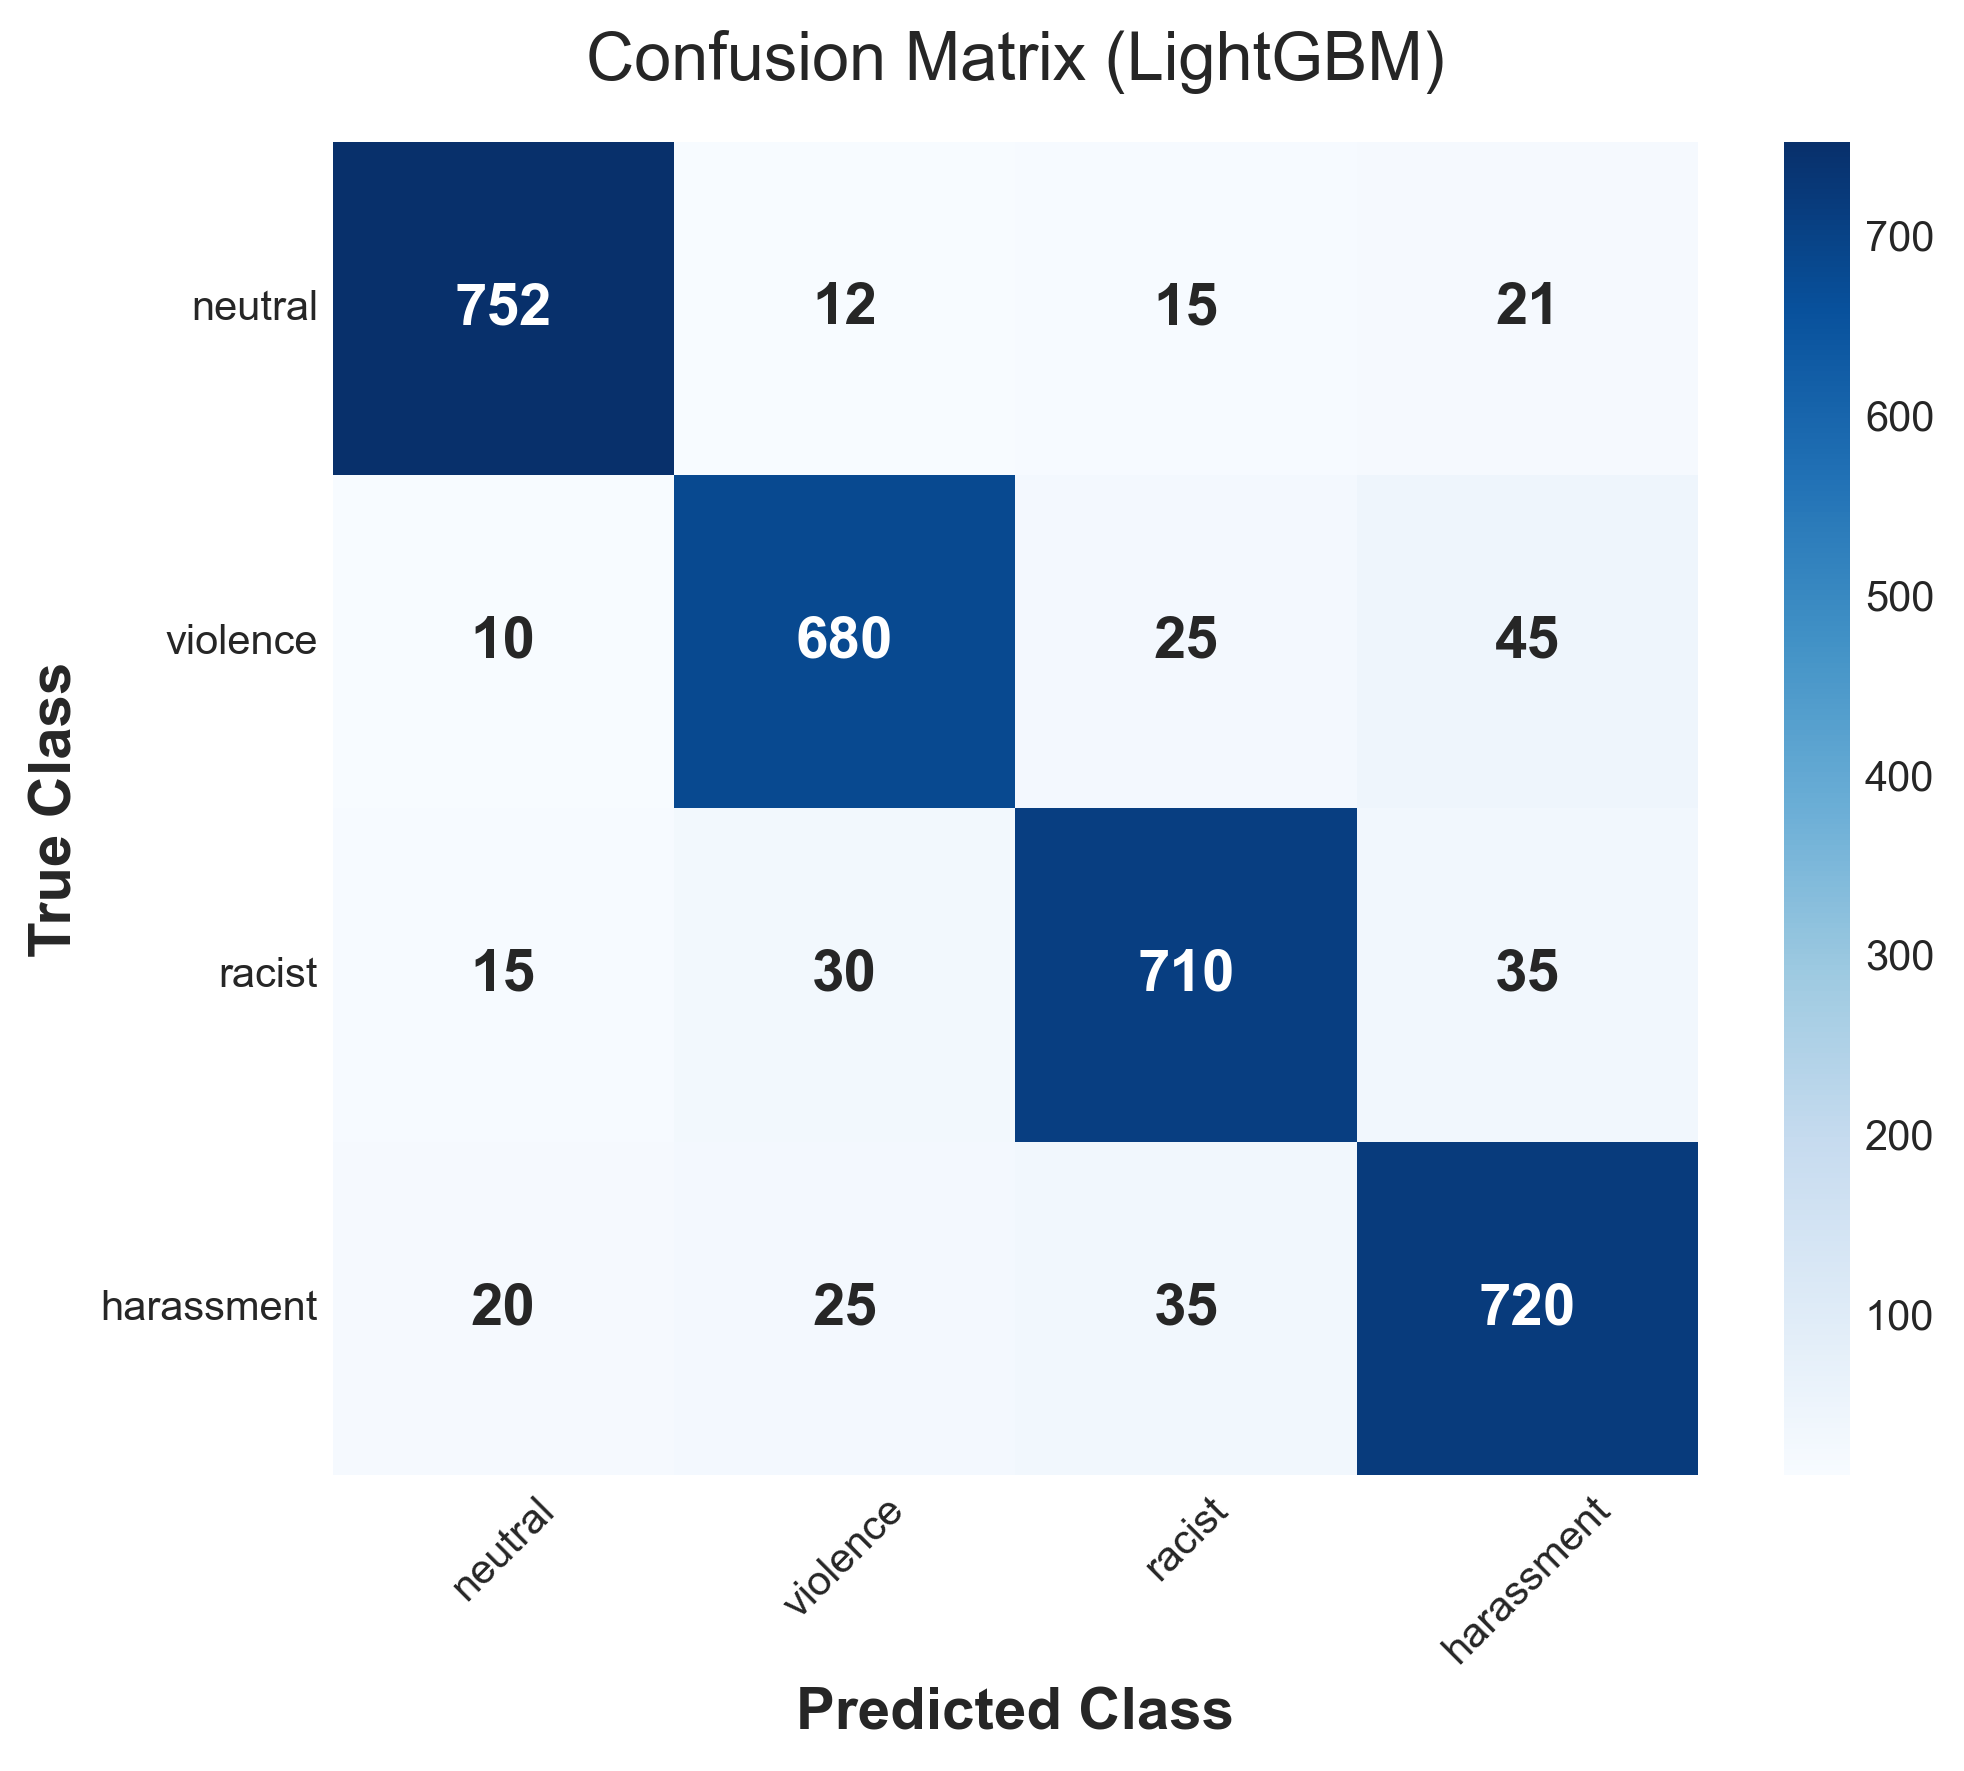
\includegraphics[height=3.8cm]{logos/dummy_cm.png}
        \end{center}
    \end{columns}
\end{frame}

\begin{frame}
    \frametitle{8. Memaksimalkan Potensi (Hyperparameter Tuning)}
    \small
    Meskipun \texttt{compare\_models()} mensortir algoritma terbaik, mesin tersebut belum mengeluarkan performa mutlaknya.
    \vspace{0.2cm}
    \begin{itemize}
        \item Sintaks komando \texttt{tune\_model(best, optimize="F1")} menyetir utilitas automasi \textit{Grid/Random Search} memutar kombinasi kenop tuas matematis arsitektur algoritma (contoh: kedalaman percabangan pohon RF, \textit{learning-rate} LightGBM).
        \item Skema \textit{tuning} menggulir silang kombinasi setelan agar mencapai titik harmonis rekor akurasi \textbf{F1-Score} setinggi mungkin di ujung jurang batas ketahanan model agar tidak \textit{overfitting}.
    \end{itemize}
\end{frame}

\begin{frame}
    \frametitle{9. Interpretability (Feature Importance)}
    \small
    Kita bisa mewawancarai alasan algoritma memvonis suatu ujaran kotor melalui \texttt{plot\_model(tuned, 'feature')}!
    \vspace{0.2cm}
    \begin{columns}[T]
        \column{0.48\textwidth}
        \begin{itemize}
            \item \textbf{Insight}: "Ternyata token kata: \textit{cina, anjing, babi, yatim, tolol} konsisten menguasai puncak peringkat koefisien matematisnya!"
            \item Jika \textit{noise stopword} (cth: "kamu") juara 1, saatnya siklus dibongkar *cleaning* ulang!
        \end{itemize}

        \column{0.48\textwidth}
        \begin{center}
            \vspace{-0.5cm}
            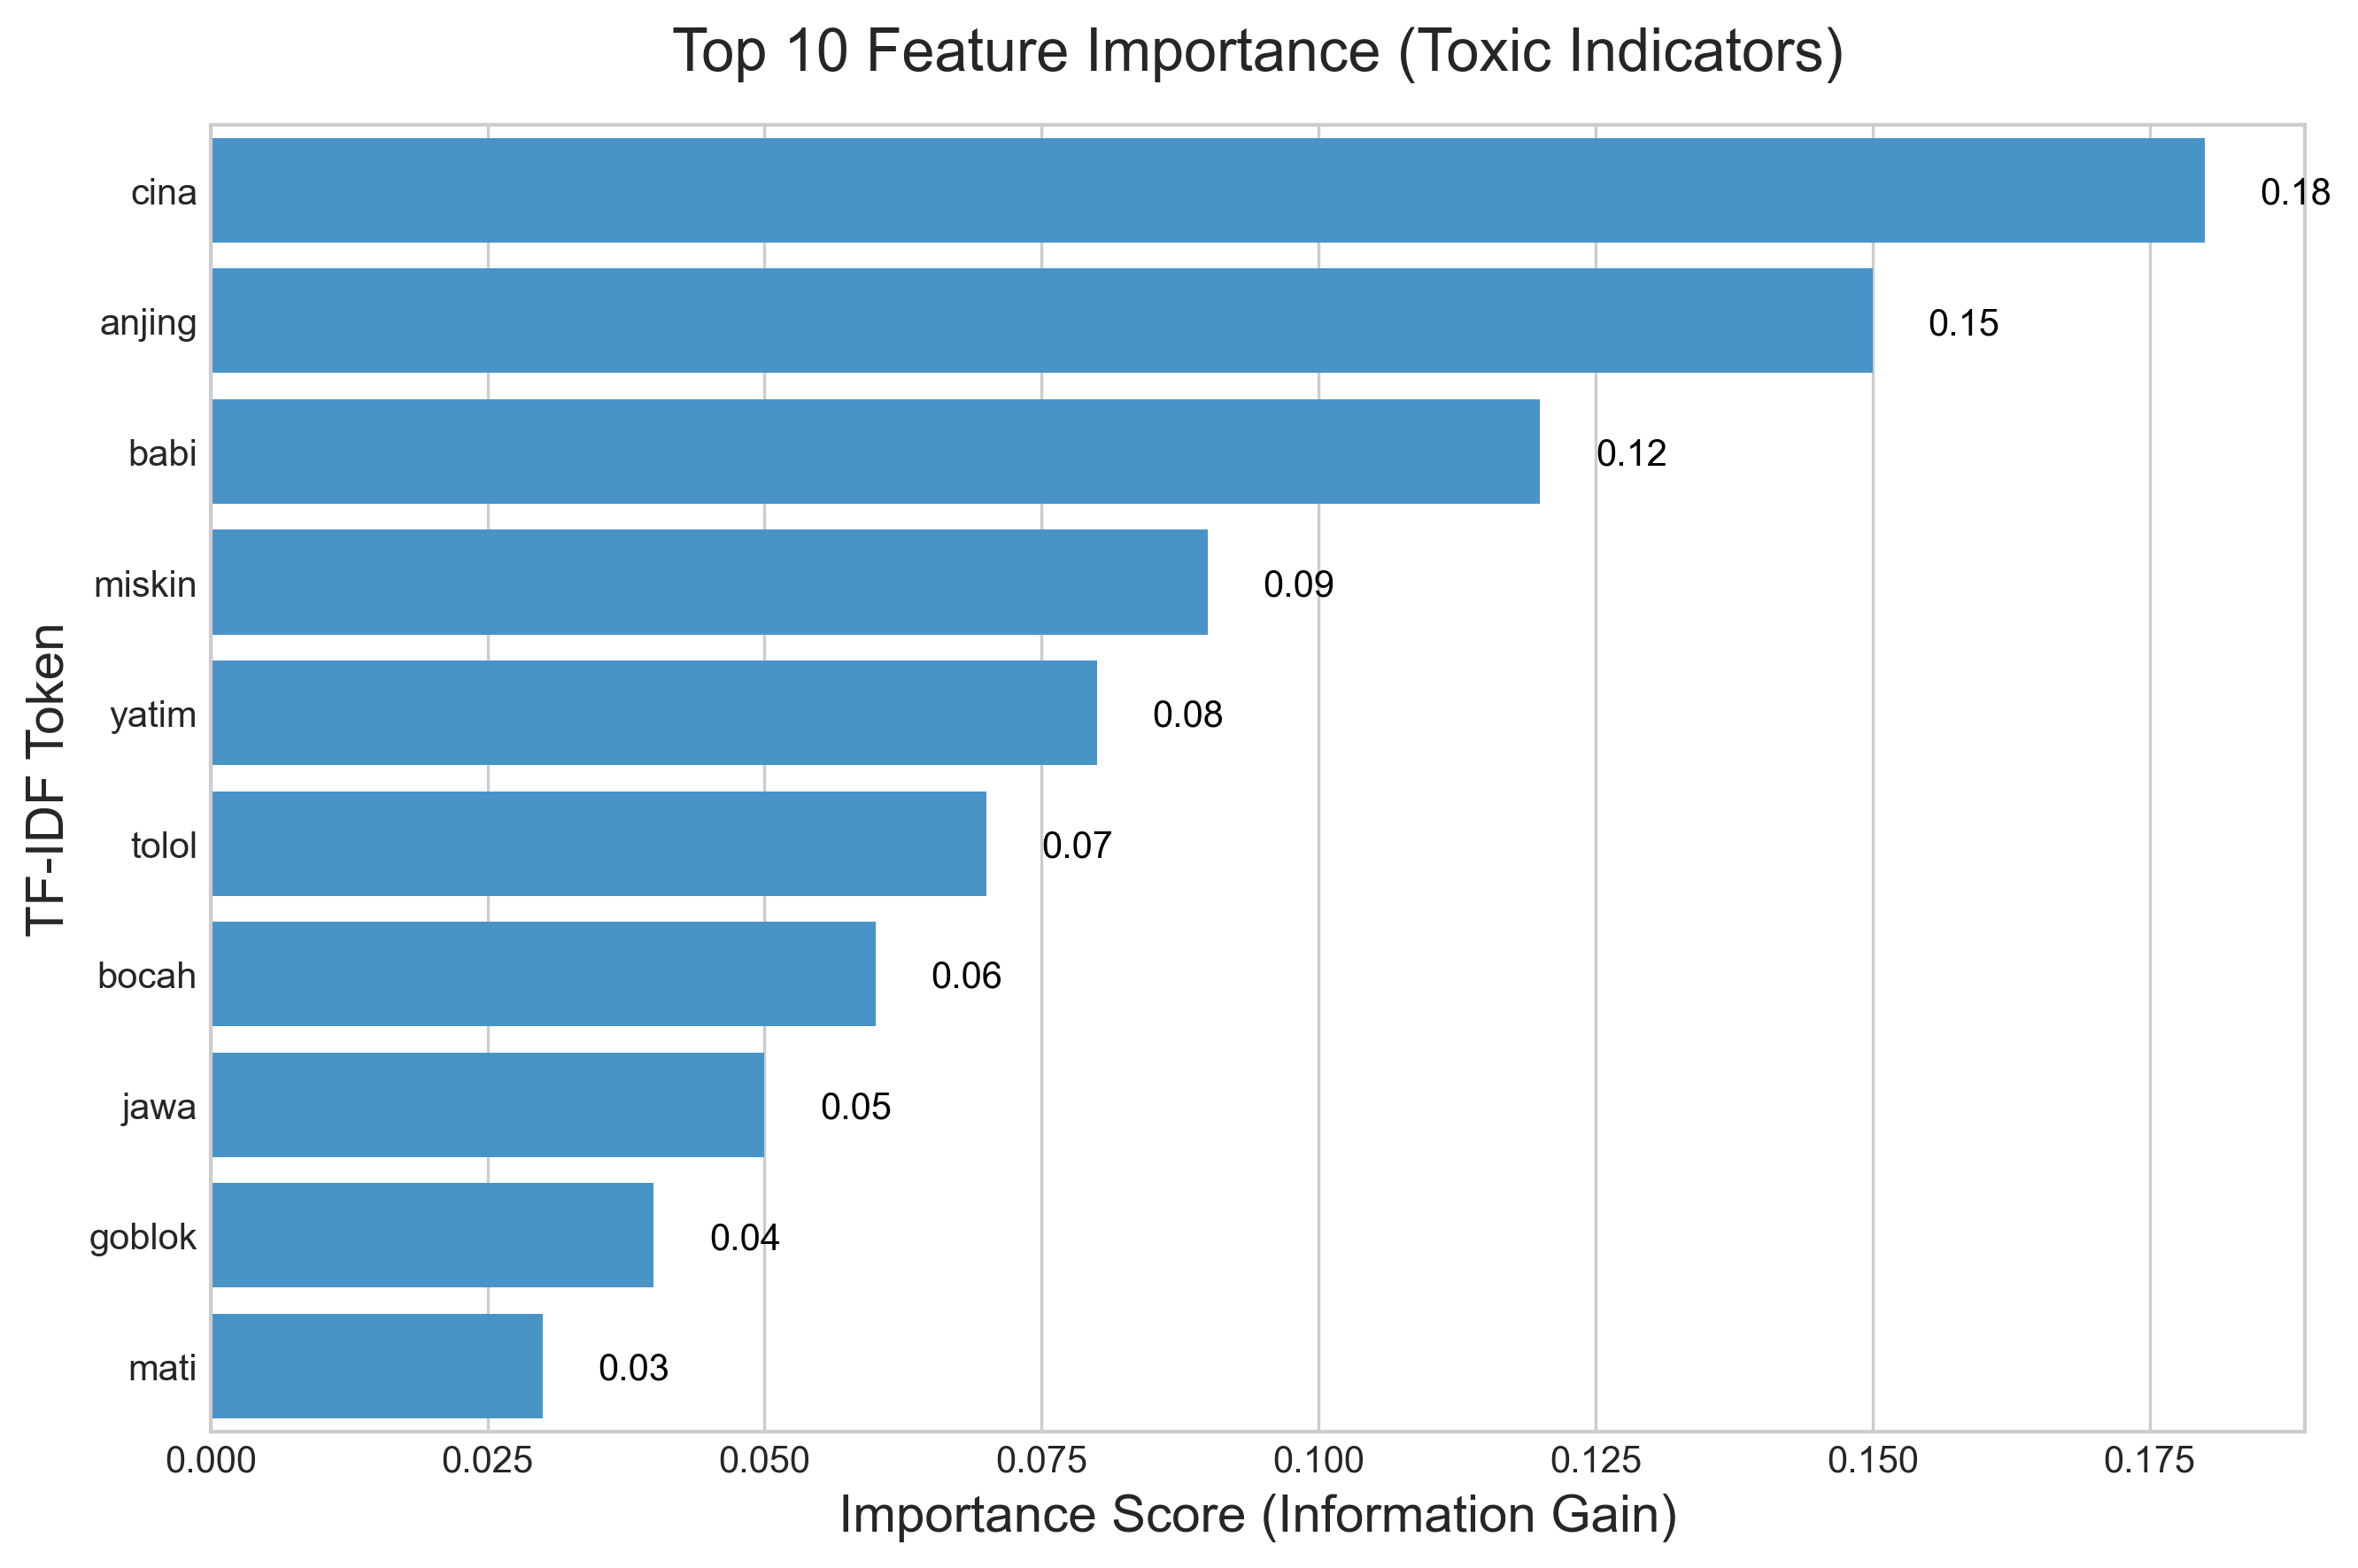
\includegraphics[height=4cm]{logos/dummy_fi.png}
        \end{center}
    \end{columns}
\end{frame}

\begin{frame}
    \frametitle{10. Finalize \& Export Model Tunggal}
    \framesubtitle{Mengawetkan "Otak" Artificial Intelligence}
    \small
    \begin{itemize}
        \item Fase pelantikan \texttt{finalize\_model(tuned)} memaksa pakem algoritma mengawinkan paksa porsi irisan \% Data Uji Rahasia (yang tabu diintip sedari awal iterasi) melebur kembali menyatu ke wadah \textit{Train}. Ia akan melahap mutlak absolut 100\% bongkahan rekaman total \textit{dataset} demi adaptabilitas terjun ke dunia siber nyata (\textit{The True Final Form}).
        \item Eksekutor kompilasi akhir \texttt{save\_model(final, 'text\_model\_v1')}  menyolder \textbf{semua perakitan kompleks multi-lapisan}: dari (1) Ekstraksi Kamus TF-IDF Teks, (2) Transformator Target One-Hot Encoder, terbungkus hingga (3) Algoritma Klasifikasi final LightGBM/RF utuh \dots ke dalam wujud file saku biner statis ekstensi \textbf{\texttt{.pkl} (Pickle)}.
    \end{itemize}
\end{frame}

\begin{frame}
    \frametitle{11. Deployment Antarmuka ke Hugging Face (1)}
    \small
    Kecerdasan *Artificial Intelligence* lumpuh fungsinya jika mustahil dipakai uji obrolan (*interactive inference*) oleh warga masyarakat awam.
    \vspace{0.2cm}
    \begin{itemize}
        \item \textbf{Hugging Face Spaces} menganugerahkan slot arsitektur komputer maya kontainer berbasis Linux gratis mengudara non-stop buat \textit{hosting} portal \textit{Machine Learning}.
        \item *Engineer* menugaskan antarmuka tatap muka elegan *low-code* menawan (*Web UI Script*) \texttt{app.py} berbasis gubahan *framework* cepat \textbf{Gradio} atau \textbf{Streamlit}.
        \item Web UI ini meresonansikan panggilan pemuatan (\textit{loading state}) *Pickle* saku resep model \texttt{.pkl} keras kita menuju aliran kesibukan *Random Access Memory* (RAM) server kontainer \textit{cloud} HF.
    \end{itemize}
\end{frame}

\begin{frame}
    \frametitle{12. Peluncuran Global HF Spaces (2)}
    \small
    \begin{itemize}
        \item Guna menjamin kontainer awan \textit{Linux Server} fasih mengoperasikan logika kita tanpa malfungsi eror, manifes daftar belanjaan resep pustaka bernomenklatur \texttt{requirements.txt} harus dinaik-sertakan.
        \item Mesin otomatis meng-unduh dan menanam persis jejak paket setara *laptop programmer*-nya (Misal mencanangkan entri paku: \texttt{pycaret==3.0.4}, \texttt{gradio}, \texttt{pandas}) tepat sesaat jelang menekan tombol hijau *Boot ON*.
        \item \textbf{Misi Paripurna}: Sedetik usai komoditas sirkuit Git *Push* terkompilasi nyala, sang pionir rekayasa NLP \textbf{resmi memiliki portal *endpoint* URL publik aplikasi sensor pendeteksi kata-kata maki *gamer* mahakaryanya mengudara ke seluruh benua planet} siap dilibas berjuta obrolan manusia!
    \end{itemize}
\end{frame}

\begin{frame}
    \frametitle{13. Hasil Deployment (Live UI)}
    \small
    \begin{center}
        \url{https://huggingface.co/spaces/mctosima/deteksi-toksisitas-chat}
        
        \vspace{0.4cm}
        % Using width instead of height to ensure the screenshot spans nicely
        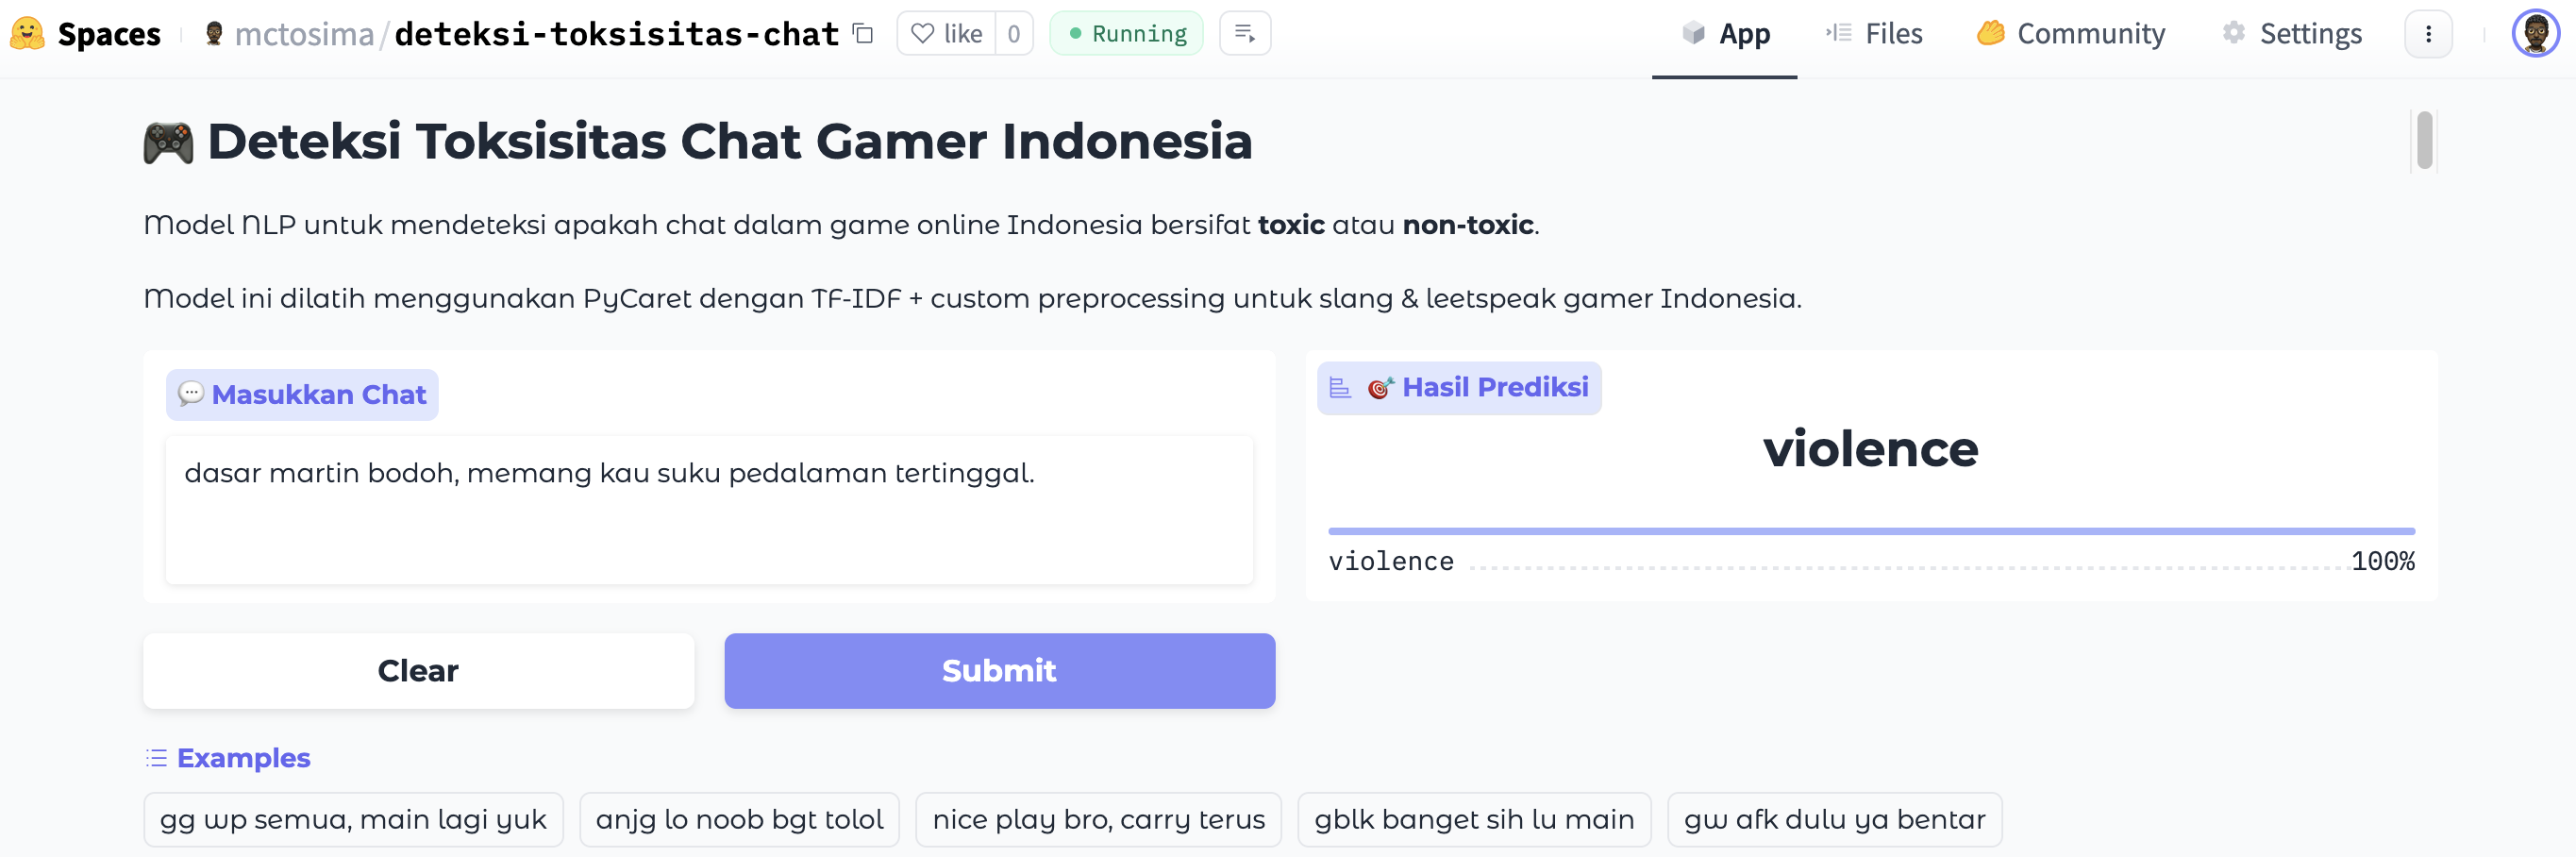
\includegraphics[width=0.9\textwidth]{contoh_hgfc.png}
    \end{center}
\end{frame}

\section{Diskusi}

\begin{frame}
    \frametitle{Mari Kita Mulai!}
    \begin{center}
        \Huge \textbf{Hands-on Time}

        \vspace{0.8cm}
        \normalsize
        Silakan buka teks editor dan \texttt{workshop\_sesi1.ipynb} kalian. Kita akan mulai dengan membuat kerangka modulenya terlebih dahulu!
    \end{center}
\end{frame}

\end{document}
